
\documentclass{standalone}
\usepackage[T1]{fontenc}
\usepackage[utf8]{inputenc}          % needed for French accents
\usepackage{pgfplotstable}
\usepackage{pgfplots}
\pgfplotsset{compat=1.18}
\usepackage{siunitx}                 % optional, nicer y‑axis numbers
\usepackage{booktabs}                % pretty tables for the optional preview

% -------------------------------------------------
% Helper that removes the internal \pgfpl@@ wrapper
% -------------------------------------------------

\begin{document}



% This file was created with matplot2tikz v0.4.0.
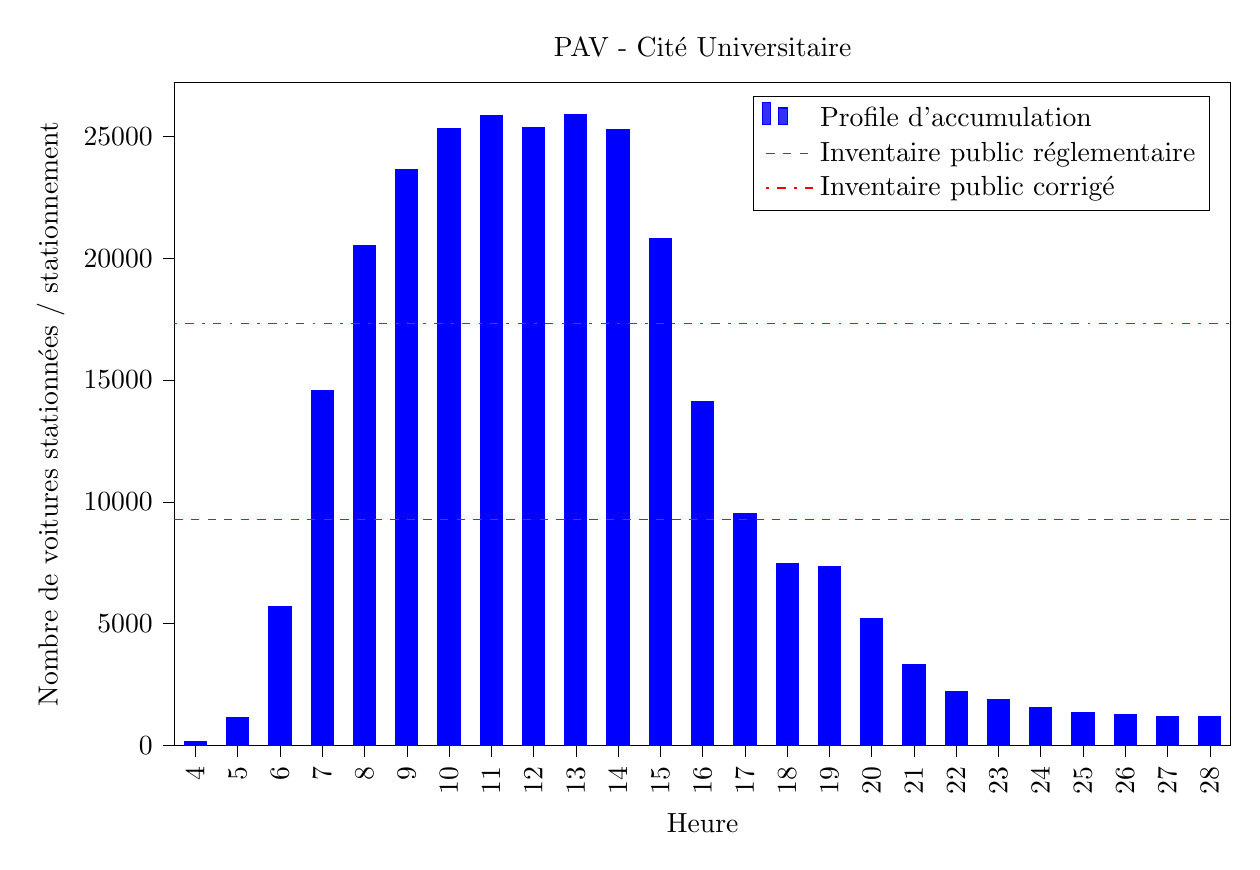
\begin{tikzpicture}

\definecolor{darkgray176}{RGB}{176,176,176}
\definecolor{lightgray204}{RGB}{204,204,204}
\definecolor{steelblue31119180}{RGB}{31,119,180}

\begin{axis}[
height=10cm,
legend cell align={left},
legend style={fill opacity=0.8, draw opacity=1, text opacity=1},
minor xtick={},
minor ytick={},
tick align=outside,
tick pos=left,
title={PAV - Cité Universitaire},
width=15cm,
xlabel={Heure},
xmin=3.5, xmax=28.5,
xtick style={color=black},
xtick={0,1,2,3,4,5,6,7,8,9,10,11,12,13,14,15,16,17,18,19,20,21,22,23,24,25,26,27,28},
xticklabel style={rotate=90.0},
ylabel={Nombre de voitures stationnées / stationnement},
ymin=0, ymax=27216,
ytick style={color=black},
ytick={0,5000,10000,15000,20000,25000,30000},
yticklabels={
  \(\displaystyle {0}\),
  \(\displaystyle {5000}\),
  \(\displaystyle {10000}\),
  \(\displaystyle {15000}\),
  \(\displaystyle {20000}\),
  \(\displaystyle {25000}\),
  \(\displaystyle {30000}\)
},
scaled ticks=false
]
\addplot[ybar,draw=blue,fill=blue,legend image post style={/pgfplots/ybar legend},
  bar width=8pt]
        coordinates{
            (4,149)
            (5,1127)
            (6,5701)
            (7,14557)
            (8,20530)
            (9,23660)
            (10,25320)
            (11,25879)
            (12,25370)
            (13,25920)
            (14,25292)
            (15,20788)
            (16,14108)
            (17,9515)
            (18,7476)
            (19,7356)
            (20,5209)
            (21,3308)
            (22,2197)
            (23,1868)
            (24,1570)
            (25,1338)
            (26,1248)
            (27,1182)
            (28,1171)};

\addlegendentry{Profile d'accumulation}
\addplot [semithick, red, dashed]
table {%
3.5 9274
28.5 9274
};
\addlegendentry{Inventaire public réglementaire }
\addplot [semithick, red, dash pattern=on 1pt off 3pt on 3pt off 3pt]
table {%
3.5 17316
28.5 17316
};
\addlegendentry{Inventaire public corrigé}
\end{axis}

\end{tikzpicture}
\end{document}